\section{Description of Components}
The components of Scatter Search template \cite{glover1998template}
consists of
specific subroutines of the following types:
\begin{itemize}
\item A Diversification Generator
\item An Improvement Method
\item A Reference Set Update Method
\item A Subset Generation Method
\end{itemize}
We described below
each of the components.

\subsection{A Diversification Generator}
To component is used to generate
a collection of diverse trial solutions,
using an arbitrary trial solution
(or seed solution) as an input.
%\begin{algorithm}
  \caption{Path Relinking Initial Phase}\label{pr_init}
  \begin{algorithmic}[0]
    \Procedure{PathRelinking}{$Instance$}
    \State $EliteSols \gets MultiStart(Instance)$
    \Repeat
    \State $MiscSols \gets GenerateMiscSols(Instance,EliteSols)$
    \ForAll{$x \in MiscSols$}
    \State $ImprovementMethod(x)$
    \State $EliteSols.Update(x)$
    \EndFor
    \Until{$PerfectMatchingCost(MiscSols,EliteSols) < \epsilon$}
    \State $SubsetControl(EliteSols)$
    \EndProcedure
  \end{algorithmic}
\end{algorithm}

In this research
we develop a Greedy Randomized Adaptive Search Procedure (GRASP)
as a diversification generator.
GRASP \cite{feo1995greedy}
is a multi-start procedure that combines
the power of greedy heuristics and randomization.

GRASP typically consists of two phases:
a greedy randomized construction phase
and an improvement phase.
In this case,
our proposed GRASP
consist only of the construction phase
because the improvement phase
is applied in other parts
of the scatter search algorithm.
\subsubsection{GRASP}
%Why did you choose GRASP?
We choose GRASP
because
in the proposed problem
any allocation of sites for adjusters
is a feasible solution,
so it was decided to give some intelligence
to this simple allocation
instead of choose
random points.
%What does it consist?
We start with a partial solution
(location of a smaller number of adjusters)
with only one adjuster allocated,
evaluate each site with the greedy function,
and choose one from the best $\alpha$ evaluations,
until each adjuster was locate.
%Which evaluation functions did you use?
Several functions were evaluated
for constructive algorithm
but because presented cooperativeness
it is difficult
to approximate the final results
in a partial solution
with a greedy function.
We use three greedy functions
to test the construction.
%Fist function
The first function,
was the p-mean
or the sum the distances
of each allocation 
from each located adjuster
with their nearest demand points.
\begin{equation}
  \label{eq:grasp1}
  \sum_{j=1}^{m}{
    \sum_{i=1}^{n}{
      t_{ij}y_{ij}^{1}
    }
  }
\end{equation}
%Second function
For the second function,
we try to incorporate cooperatively,
including in the evaluation
the distance of allocations
from each located adjuster,
with their $k$ nearest demand points
plus \textit{idle} probability
given that is allocated
to their $k-1$ nearest demand points.
\begin{equation}
  \label{eq:grasp2}
  \sum_{j=1}^{m}{
    \sum_{k=1}^{p}{
      \sum_{i=1}^{n}{
        h_{ij}^{k}t_{ij}y_{ij}^{k}
      }
    }
  }
\end{equation}
%Third function
The third function,
consist in use the Mean Service Time (MST) calibration method
proposed by Jarvis \cite{jarvis1985approximating},
to obtain more accuracy values
of the current mean response time.


\subsection{An Improvement Method}
The goal of this component
is to transform a trial solution
into one or more enhanced trial solutions. 
If no improvement
of the input trial solution results, 
the ``enhanced'' solution
is considered to be
the same as the input solution.

We developed two improvement methods,
the first one is an adaptation
of the method proposed by Berman et al. \cite{berman1987stochastic}
(see Appendix \ref{ch:Berman} for mode details)
and the second one,
a Local Search
described in the next section.
%\todo[inline]{Incluir descripcion del metodo de Berman}
\subsection{Proposed Local Search}
%the move
The move considered
is to relocate an agent from its current position
to a different position.
%the neighborhood
The entire neighborhood
consist of all possible moves
that can take place from a given solution.
However,
due to the high cost of move relocation assessment,
a reduced neighborhood is considered.
Thus,
instead of considering all possible moves,
the procedure focuses on relocating the adjuster
with the smallest workload
to a place around or near the adjuster with the largest workload.
\missingfigure[figwidth=6cm]{Example of less workload adjuster}
\missingfigure[figwidth=6cm]{Example of neighborhood to evaluate}


\subsection{A Reference Set Update Method}
This method is used
to build and maintain a Reference Set
consisting of the \textit{b} best solutions found
(where the value of \textit{b}
is typically small,
e.g., between 20 and 40),
organized in an array
to provide efficient accessing
by other parts of the method.

We choose
a two level Reference Set
to maintain
good quality solutions
and diverse solutions.
This is
because the combination method
generates similar solutions as the input,
%And we opt for be dynamic
%since the number
%of generated solutions
%is big (proportional to \textit{p}).
and Moreover,
the size of the reference set is dynamically determined,
according to $p$.

Whenever the Reference Set is update
with a set of solutions
%\todo{No se entiende!}
the update method
first try to incorporate the solutions
by quality criteria;
%because the Reference Set is divided
%in two parts,
%first try to accommodate each solution
if a solutions enters the Reference Set,
degrades a lower quality solution,
removing the worst solution of the Reference Set.
These steps are shown in Algorithm \ref{alg:rs_update}.
\begin{algorithm}
  \caption{Reference Set Update Method}\label{alg:rs_update}
  \begin{algorithmic}[0]
    \Procedure{ReferenceSet.Update}{$ToUpdateSols$}
    \State $Bin \gets PublicBin()$
    \For{$Sol \in ToUpdateSols$}
    \If{$Sol.Quality > RefSet.LowestQuality$}
    \State $DegradedSol \gets RefSet.LowestQualitySol()$
    \State $RefSet.Remove(DegragedSol)$
    \State $RefSet.InsertByQuality(Sol)$
    \State $Bin.Add(DegradedSol)$
    \Else
    \State $Bin.Add(Sol)$
    \EndIf \EndFor
    \EndProcedure
  \end{algorithmic}
\end{algorithm}


After adding solutions to the Reference Set
by using the quality criterion,
% Update Diversity
every solution that was generated
and did not enter the Reference Set,
displaced by a better solution,
or actually
a member of the diverse part of the Reference Set
is evaluated to be in the Reference Set
as a diverse solution.
As shown by the Algorithm \ref{alg:rs_updatediv}.
\begin{algorithm}
  \caption{Reference Set Update Diversity Method}
  \label{alg:rs_updatediv}
  \begin{algorithmic}[0]
    \Procedure{ReferenceSet.UpdateDiversity}{}
    \State $Bin \gets PublicBin()$
    \State $Bin \gets Bin \cup RefSet.DiversitySols()$
    \State $RefSet.Remove(RefSet.DiversitySols())$
    \For{$Sol \in Bin$}
    \State $Sol.DiversityValue \gets MinumumCostPerfectMatching(RefSet,Sol)$
    \EndFor
    \Repeat
    \State $DiverseSol \gets MostDiverse(Bin)$
    \State $Bin.Remove(DiverseSol)$
    \State $RefSet.InsertByDiversity(DiverseSol)$
    \For{$Sol \in Bin$}
    \State $Sol.UpdateDiversityValue(DiverseSol)$
    \EndFor
    \Until{$Count(RefSet.DiversitySols()) = b$ \textbf{or} $Count(Bin) = 0$}
    \EndProcedure
  \end{algorithmic}
\end{algorithm}

%solutions that do not enter the Reference Set
%and those that have been removed,
%are considered to be part
%of the Reference Set
%by using the diversity criterion.
%reassessing the diverse solutions,
%since they evaluation depends
%on the quality members.
%\todo[inline]{Agregar como se mide la diversidad}
%% We need layers to draw the block diagram
\pgfdeclarelayer{background}
\pgfdeclarelayer{foreground}
\pgfsetlayers{background,main,foreground}

% Define a few styles and constants
\tikzstyle{sensor}=[draw, fill=blue!20, text width=5em, 
  text centered, minimum height=2.5em]
\tikzstyle{ann} = [above, text width=5em]
\tikzstyle{naveqs} = [sensor, text width=6em, fill=red!20, 
  minimum height=12em, rounded corners]
\def\blockdist{2.3}
\def\edgedist{2.5}

\begin{figure}
  \label{fig:SS_Upd}
  \centering
  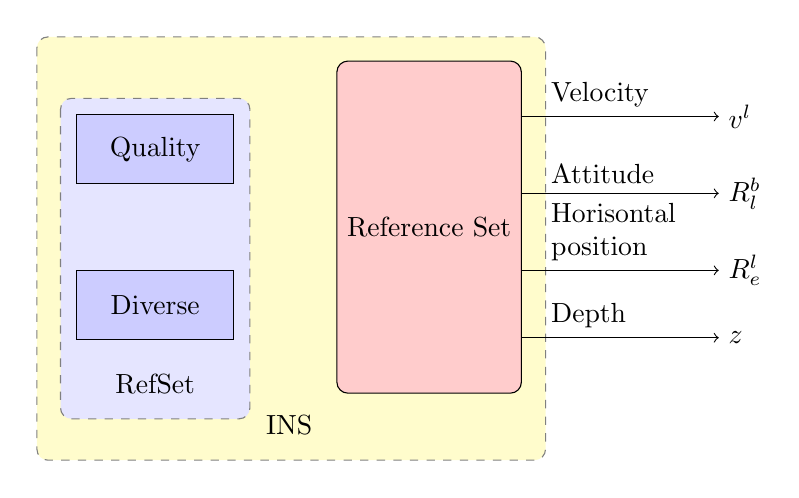
\begin{tikzpicture}
    \node (naveq) [naveqs] {Reference Set};
    % Note the use of \path instead of \node at ... below. 
    \path (naveq.140)+(-\blockdist,0) node (gyros) [sensor] {Quality};
    \path (naveq.-140)+(-\blockdist,0) node (accel) [sensor] {Diverse};
    
    %    \path [draw, ->] (gyros) -- node [above] {$\vc{\omega}_{ib}^b$} 
    %    (naveq.west |- gyros) ;
    % We could simply have written (gyros) .. (naveq.140). However, it's
    % best to avoid hard coding coordinates
    %      \path [draw, ->] (accel) -- node [above] {$\vc{f}^b$} 
    %      (naveq.west |- accel);
    \node (IMU) [below of=accel] {RefSet};
    \path (naveq.south west)+(-0.6,-0.4) node (INS) {INS};
    \draw [->] (naveq.50) -- node [ann] {Velocity } + (\edgedist,0) 
    node[right] {$\vc{v}^l$};
    \draw [->] (naveq.20) -- node [ann] {Attitude} + (\edgedist,0) 
    node[right] { $\mx{R}_l^b$};
    \draw [->] (naveq.-25) -- node [ann] {Horisontal position} + (\edgedist,0)
    node [right] {$\mx{R}_e^l$};
    \draw [->] (naveq.-50) -- node [ann] {Depth} + (\edgedist,0) 
    node[right] {$z$};
    
    % Now it's time to draw the colored IMU and INS rectangles.
    % To draw them behind the blocks we use pgf layers. This way we  
    % can use the above block coordinates to place the backgrounds   
    \begin{pgfonlayer}{background}
      % Compute a few helper coordinates
      \path (gyros.west |- naveq.north)+(-0.5,0.3) node (a) {};
      \path (INS.south -| naveq.east)+(+0.3,-0.2) node (b) {};
      \path[fill=yellow!20,rounded corners, draw=black!50, dashed]
      (a) rectangle (b);
      \path (gyros.north west)+(-0.2,0.2) node (a) {};
      \path (IMU.south -| gyros.east)+(+0.2,-0.2) node (b) {};
      \path[fill=blue!10,rounded corners, draw=black!50, dashed]
      (a) rectangle (b);
    \end{pgfonlayer}
  \end{tikzpicture}
  \caption{Scatter Search Update Method}
\end{figure}
\todo{Ajustar imagen si es que se va a dejar}


\subsection{A Subset Generation Method}
This component operates on the Reference Set,
%to produce a subset of its solutions
%as a basis for creating combined solutions.
it is used to create subsets
of solutions that are combined
by the Combination Method.
\begin{algorithm}
  \caption{Subsets Generator}\label{alg:subsets}
  \begin{algorithmic}[0]
    \Procedure{GenerateSubsets}{$RefSet,NowTime$}
    \State $NewSols \gets RefSet.SolutionsSince(NowTime)$
    \ForAll{$(Sol_x,Sol_y) \in NewSols$}
    \If{$Sol_x \in RefSet$ \textbf{and} $Sol_y \in RefSet$}
    \State $CombinedSols \gets PathRelinkingCombination(Sol_x,Sol_y)$
    \State $RefSet.Update(CombinedSols)$
    \EndIf \EndFor
    \State $RefSet.UpdateDiversity()$
    \If{$RefSet.NumberOfOldSols(NowTime) > 0$}
    \State $OldSols \gets RefSet.SolutionsUntil(NowTime)$
    \ForAll{$Sol_x \in NewSols$}
    \ForAll{$Sol_y \in OldSols$}
    \If{$Sol_x \in RefSet$ \textbf{and} $Sol_y \in RefSet$}
    \State $CombinedSols \gets PathRelinkingCombination(Sol_x,Sol_y)$
    \State $RefSet.Update(CombinedSols)$
    \EndIf \EndFor
    \State $RefSet.UpdateDiversity()$
    \EndFor \EndIf
    \EndProcedure
  \end{algorithmic}
\end{algorithm}

We only look for subsets of size two,
i.e. pairs of solutions;
because our Reference Set is dynamic,
at the beginning of each iteration
we label the solutions as new and old
to identify them,
and avoid create pairs previous combined.
To generate the pairs
we use
a new solution with another new solution,
%\todo{Refrasear}
after
if there are old solutions
we make pairs
with a new solution
and an old solution.

Is important to notice that
the new solutions that enters in the Reference Set
at the current iteration
are not part of the subsets
until the next iteration.

\subsection{A Solution Combination Method}
With this component,
our scatter search
transforms a given subset of solutions 
produced by the Subset Generation Method
into
one or more combined solution vectors.

We choose a path relinking as a combination method
consisting of
determining a match between servers,
this match can be
\begin{itemize}
\item Perfect Matching:
  minimizing the distance between paired servers
\item Workload Matching:
  sorting the servers of both solutions
  according to their workload,
  and match them according to these sorted lists.
\item Random Matching
\end{itemize}
Once we have the matching
we proceed from one solution
to interchange each server,
one by one
until the other solution is reached;
in each interchange
we have a new solution.
To make the interchanges
we have three options:
\begin{itemize}
\item Nearest First
\item Farthest First
\item Random
\end{itemize}
\begin{algorithm}
  \caption{Path Relinking Combination Method}\label{alg:pr_combination}
  \begin{algorithmic}[0]
    \Procedure{PahtRelinkingCombination}{$Sol_x,Sol_y$}
    \State $CombinedSols \gets EmptyList()$
    \State $match \gets Matching(Sol_x,Sol_y)$
    \Comment{perfect,workload,random}
    \State $order \gets ProcessOrder(Sol_x,match,Sol_y)$
    \Comment{nearest/farthest first,random}
    \For{$i \gets 1,p$}
    \State $j \gets order[i]$
    \If{$Sol_x.ServerLocation(j) != Sol_y.ServerLocation(match[j])$}
    \State $Sol_x.SetServerLocation(j,Sol_y.ServerLocation(match[j]))$
    \State $CombinedSols.insert(Sol_x)$
    \EndIf \EndFor
%    \State \textbf{return} $CombinedSols$
    \EndProcedure
  \end{algorithmic}
\end{algorithm}

%\todo[inline]{Hacer mas claro la secuencia y metodos}
